%*******************************************************************************
%****************************** Second Chapter *********************************
%*******************************************************************************

\chapter{Implementations}

\ifpdf
    \graphicspath{{Chapter5/Figs/Raster/}{Chapter5/Figs/PDF/}{Chapter5/Figs/}}
\else
    \graphicspath{{Chapter5/Figs/Vector/}{Chapter5/Figs/}}
\fi

\section{Architecture}

\begin{figure}[h!] 
\centering    
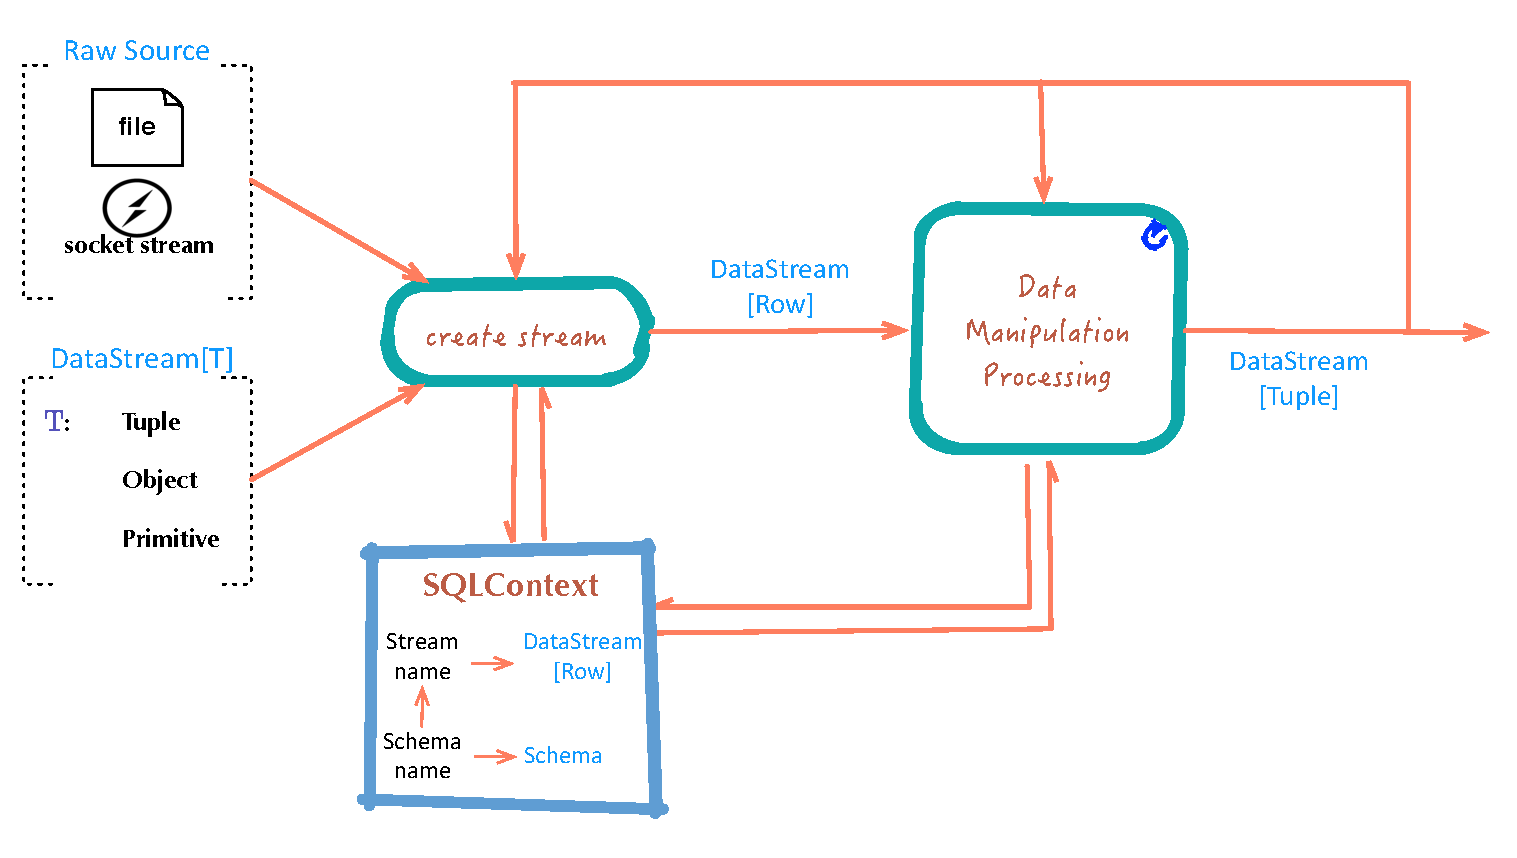
\includegraphics[width=1\textwidth]{Architecture}
\caption{Architecture}
\label{fig:Architecture}
\end{figure}


Figure~\ref{fig:Architecture} depicts the overall architecture of FlinkCQL query processing layer. It accepts data streams, query string and SQLContext as inputs and return one or more output data streams.
\subsection{Input Sources}
The query processing layer can connect to and process data streams from different data sources like file sources, web sockets, message queues (Apache Kafka, RabbitMQ, Twitter Streaming API …), and also from any user defined data sources. We classify the sources into 2 categories: \textit{Raw source} and predefined \textit{DataStream[T]} with \textit{T} is the type of elements.

\subsubsection*{Raw Source}


\textbf{Text file stream}: the source stream contains the lines of the files created (or modified) in a given directory. The system continuously monitors the given path, and processes any new files or modifications. The file will be read with the system’s default character set. FlinkCQL expresses the text file stream source via ``SOURCE FILE ( \textit{filePath, delimiter})'', the default delimiter is a comma. The delimiter is used to tokenize string and convert its result into tuples according to a schema


\textbf{Socket text stream}: the source stream contains the strings received from the given socket. Strings are decoded by the system’s default character set. Socket text stream is specified in FlinkCQL as ``SOURCE SOCKET ( \textit{filePath, delimiter})''
The user can optionally set a delimiter for the same purpose as in Text file stream.


\textbf{Message queue connectors:} There are pre-implemented connectors for a number of popular message queue services. Connectors provide an interface for accessing data from various third party sources (message queues). Currently three connectors are natively supported, namely Apache Kafka, RabbitMQ and the Twitter Streaming API. In the recent prototype of FlinkCQL, we have not designed any syntax for those connectors due to lacking of testing facilities. However, in the next prototype, we could extend its syntax at ease.

\subsection{SQL Context}


\subsection{Query Processing}

\subsection{Output Data Streams}

// accept multiple input

\section{Query Interpreter}
\begin{figure}[h!] 
\centering    
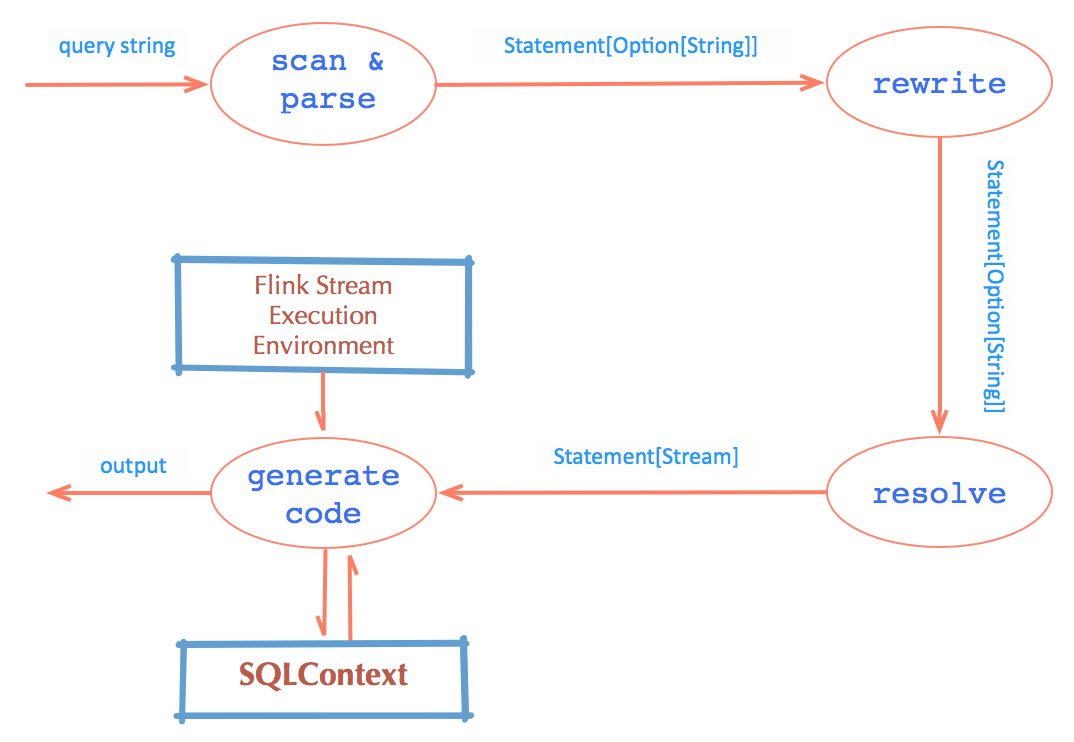
\includegraphics[width=0.7\textwidth]{QueryProcessing}
\caption{Query Processing}
\label{fig:QueryProcessing}
\end{figure}



\subsection{Parsing}

\begin{figure}[h!] 
\centering    
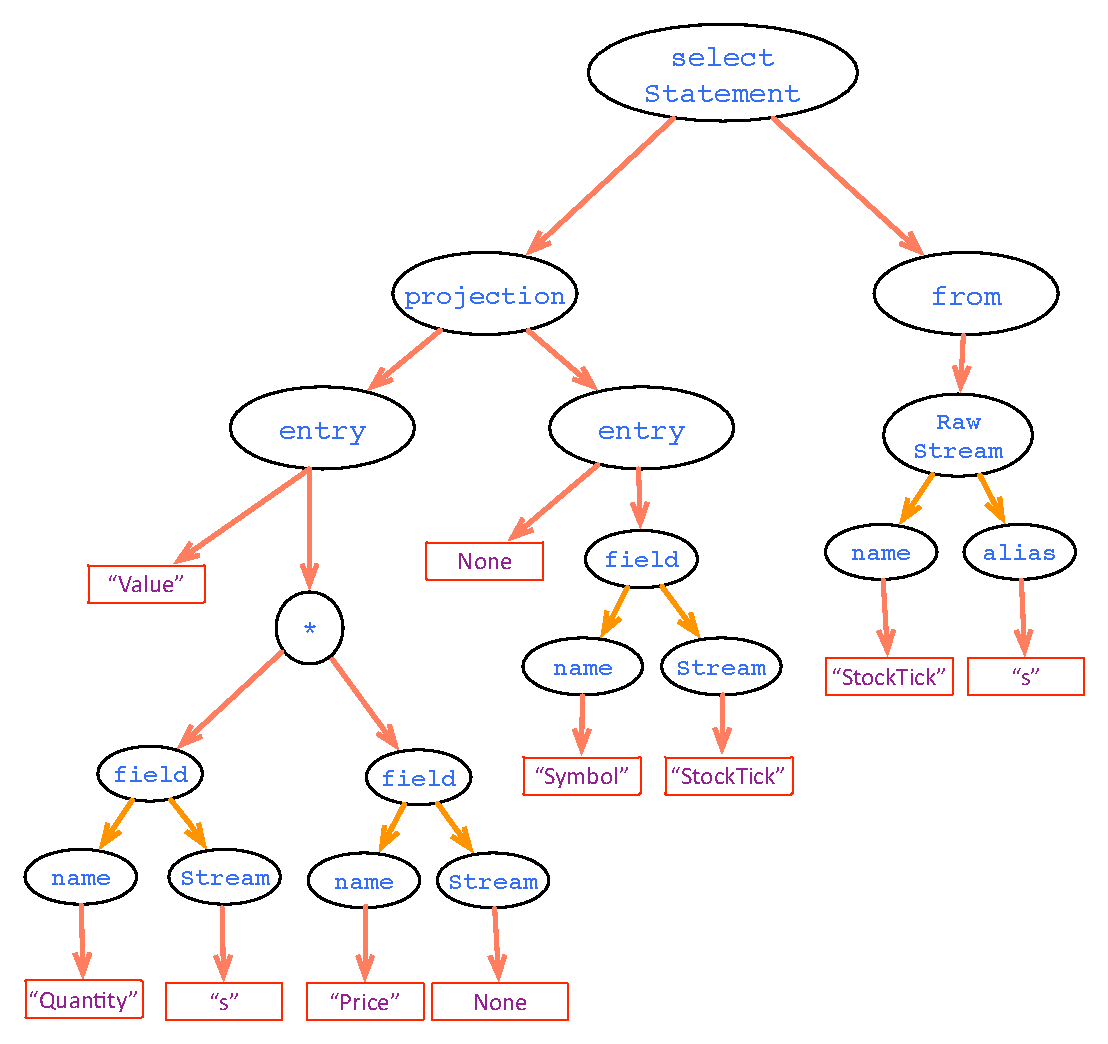
\includegraphics[width=0.7\textwidth]{Parse}
\caption{Parse}
\label{fig:Parse}
\end{figure}

At vero eos et accusamus et iusto odio dignissimos ducimus qui blanditiis praesentium voluptatum deleniti atque corrupti quos dolores et quas molestias excepturi sint occaecati cupiditate non provident, similique sunt in culpa qui officia deserunt mollitia animi, id est laborum et dolorum fuga. Et harum quidem rerum facilis est et expedita distinctio. Nam libero tempore, cum soluta nobis est eligendi optio cumque nihil impedit quo minus id quod maxime placeat facere possimus, omnis voluptas assumenda est, omnis dolor repellendus. Temporibus autem quibusdam et aut officiis debitis aut rerum necessitatibus saepe eveniet ut et voluptates repudiandae sint et molestiae non recusandae. Itaque earum rerum hic tenetur a sapiente delectus, ut aut reiciendis voluptatibus maiores alias consequatur aut perferendis doloribus asperiores repellat

\subsection{Resolving}
\begin{figure}[h!] 
\centering    
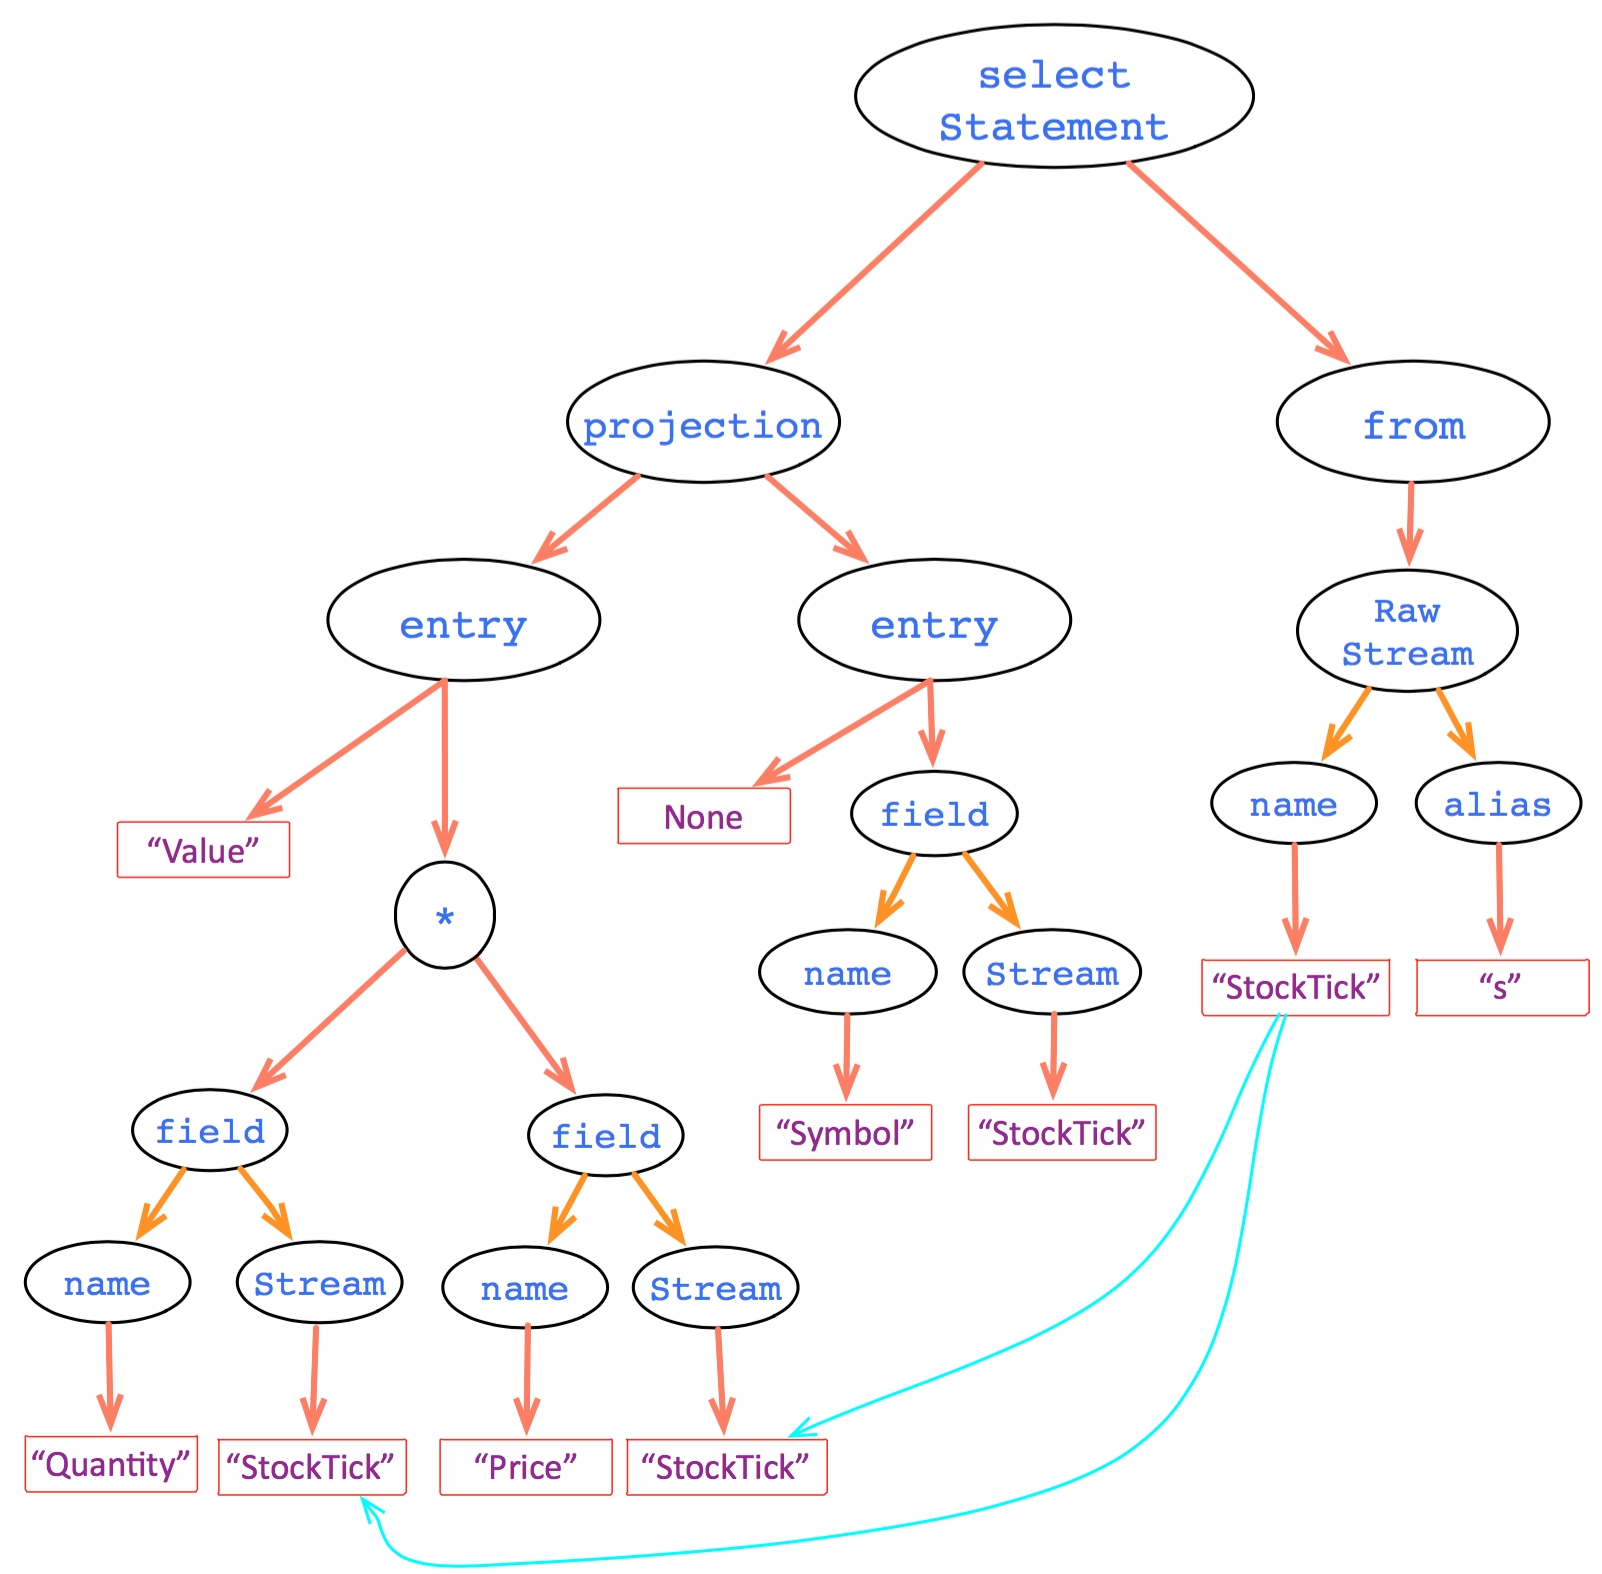
\includegraphics[width=0.7\textwidth]{Resolve}
\caption{Resolve}
\label{fig:Resolve}
\end{figure}

At vero eos et accusamus et iusto odio dignissimos ducimus qui blanditiis praesentium voluptatum deleniti atque corrupti quos dolores et quas molestias excepturi sint occaecati cupiditate non provident, similique sunt in culpa qui officia deserunt mollitia animi, id est laborum et dolorum fuga. Et harum quidem rerum facilis est et expedita distinctio. Nam libero tempore, cum soluta nobis est eligendi optio cumque nihil impedit quo minus id quod maxime placeat facere possimus, omnis voluptas assumenda est, omnis dolor repellendus. Temporibus autem quibusdam et aut officiis debitis aut rerum necessitatibus saepe eveniet ut et voluptates repudiandae sint et molestiae non recusandae. Itaque earum rerum hic tenetur a sapiente delectus, ut aut reiciendis voluptatibus maiores alias consequatur aut perferendis doloribus asperiores repellat

\subsection{Query Rewriting}
\subsection{Code Generation}


\section{Evaluations}

Compare to other systems


\section{Future Works}


http://www.sqlstream.com/blog/2015/03/5-reasons-why-spark-streamings-batch-processing-of-data-streams-is-not-stream-processing/



Data Input
http://flink.apache.org/news/2015/05/11/Juggling-with-Bits-and-Bytes.html


http://ci.apache.org/projects/flink/flink-docs-master/internals/fig/stack.svg

http://ci.apache.org/projects/flink/flink-docs-master/internals/general\_arch.html